\documentclass[../calc1-main.tex]{subfiles}

\begin{document}

\begin{example}
  Find the area of the largest rectangle that can be inscribed in a semicircle of radius R if one side of the rectangle lies along the diameter of the semicircle.

\end{example}

\begin{minipage}{0.5\textwidth}
  \begin{solution}
    $(x/2)^2 + y^2 = R^2$. So
    \[
      A = x y = x \sqrt{R^2 - (x/2)^2}.
    \]
    \[
      \frac{dA}{dx} = \frac{2R^2 - x^2}{\sqrt{4R^2-x^2}}
    \]
    The derivative is zero when $x=\sqrt{2}R$. Use the first derivative test to see that this gives max area $A = R^2$.
  \end{solution}
\end{minipage}%
\begin{minipage}{0.5\textwidth}
  \centering
  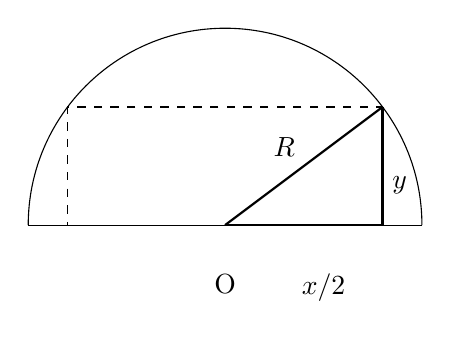
\begin{tikzpicture}[scale=2.5]
    \draw (1,0) arc [radius=1, start angle=0, end angle= 180];
    \draw[dashed] (0.8,0)--(0.8,0.6)--(-0.8,0.6)--(-0.8,0);
    \draw[thick] (0,0) -- (0.8, 0);
    \draw[thick] (0.8,0) -- (0.8, 0.6);
    \draw[thick] (0,0) -- (0.8, 0.6);
    \draw (-1,0) -- (1, 0);
    \node[below] at (0,-.2) {O};
    \node[below] at (0.5, -.2) {$x/2$};
    \node[right] at (0.8, 0.2) {$y$};
    \node[above] at (0.3, 0.3) {$R$};
  \end{tikzpicture}
\end{minipage}

\begin{example}
  Find the shortest distance from the origin to the curve $x^2 y^4 = 1$.
\end{example}
\begin{solution}
  The distance is $\sqrt{x^2} + y^2$. Instead of minimizing distance, an easier way is to minimize its square $x^2 + y^2$. Solving $x^2 y^4 = 1$ for $y$ and plugging into distance,
  \[
    D(y) = \frac{1}{y^4} + y^2
  \]
  Then $D'(y) = -\frac{4}{y^5} + 2y$. Solving $D'(y) = 0$ for $y$ we get $y = 2^{1/6}$. Use the first derivative test to check that $D(2^{1/6}) = \frac{3}{\sqrt[3]{8}}$ is a minimum.
\end{solution}

\begin{example}
  A manufacturer has 100 tons of metal that he can sell now with a profit of \$5 a ton.  For each week that he delays shipment, he can produce another 10 tons of metal.  However, for each week he waits, the profit drops 25 cents a ton.  If he can sell the metal at any time, when is the best time to sell so that his profit is maximized?
\end{example}
\begin{solution}
  Let $x$ be the number of weeks to wait.
  \begin{table}[H]
    \centering
    \begin{tabular}{|c|c|c|c|}
      \hline
      Ship & Amount of metal & Profit per ton & Total profit \\
      \hline
      now & 100 & 5 & 500 \\
      in x weeks & $100+10x$ & $5-0.25 x$ & $500+25x-0.25 x^2$\\
      \hline
    \end{tabular}
  \end{table}
  $P(x) = 500 + 25x - 2.5x^2$. Solve $P'(x) = 0$ to find $x=5$. And maximum profit is $\$562.50$.
\end{solution}

\rule{\textwidth}{1pt}
\begin{multicols}{2}
\begin{exercise}
~\\
  \begin{enumerate}
    \item Find the shortest distance from the point $(8,1)$ to the curve $y=1+x^{3/2}$.

    Answer: $\sqrt{44}$
    \item Find the largest possible \textit{perimeter} of the  rectangle that can be inscribed in a semicircle of radius R if one side of the rectangle lies along the diameter of the semicircle.

    Answer: $\frac{10 R}{\sqrt{5}}$
    \item Among all rectangles of perimeter P, show that the square has the greatest area.
    \item Among all rectangles of given area A, show that the square has the least perimeter.
    \item Find the equation of the straight line of maximum slope tangent to the curve $y=1+2x-x^3$.

    Answer: $y=1+2x$
  \end{enumerate}
\end{exercise}
\end{multicols}
\rule{\textwidth}{1pt}

\end{document}
